\subsection{Arquetipos de Integración}

Las equivalencias entre tipos de datos y el proceso automatizado permiten crear los arquetipos de integración basados en las clases CLUSTER y ELEMENT. Estos arquetipos de integración tienen el propósito principal de ser el punto de entrada de proceso de conversión semántico para importación de datos a sistemas openEHR. La Figura \ref{fig:comparison} muestra de lado a lado un extracto de un arquetipo de integración de paciente creado utilizando el proceso automatizado y el recurso FHIR Paciente del cual se creo.

\begin{figure*}
  \centering
  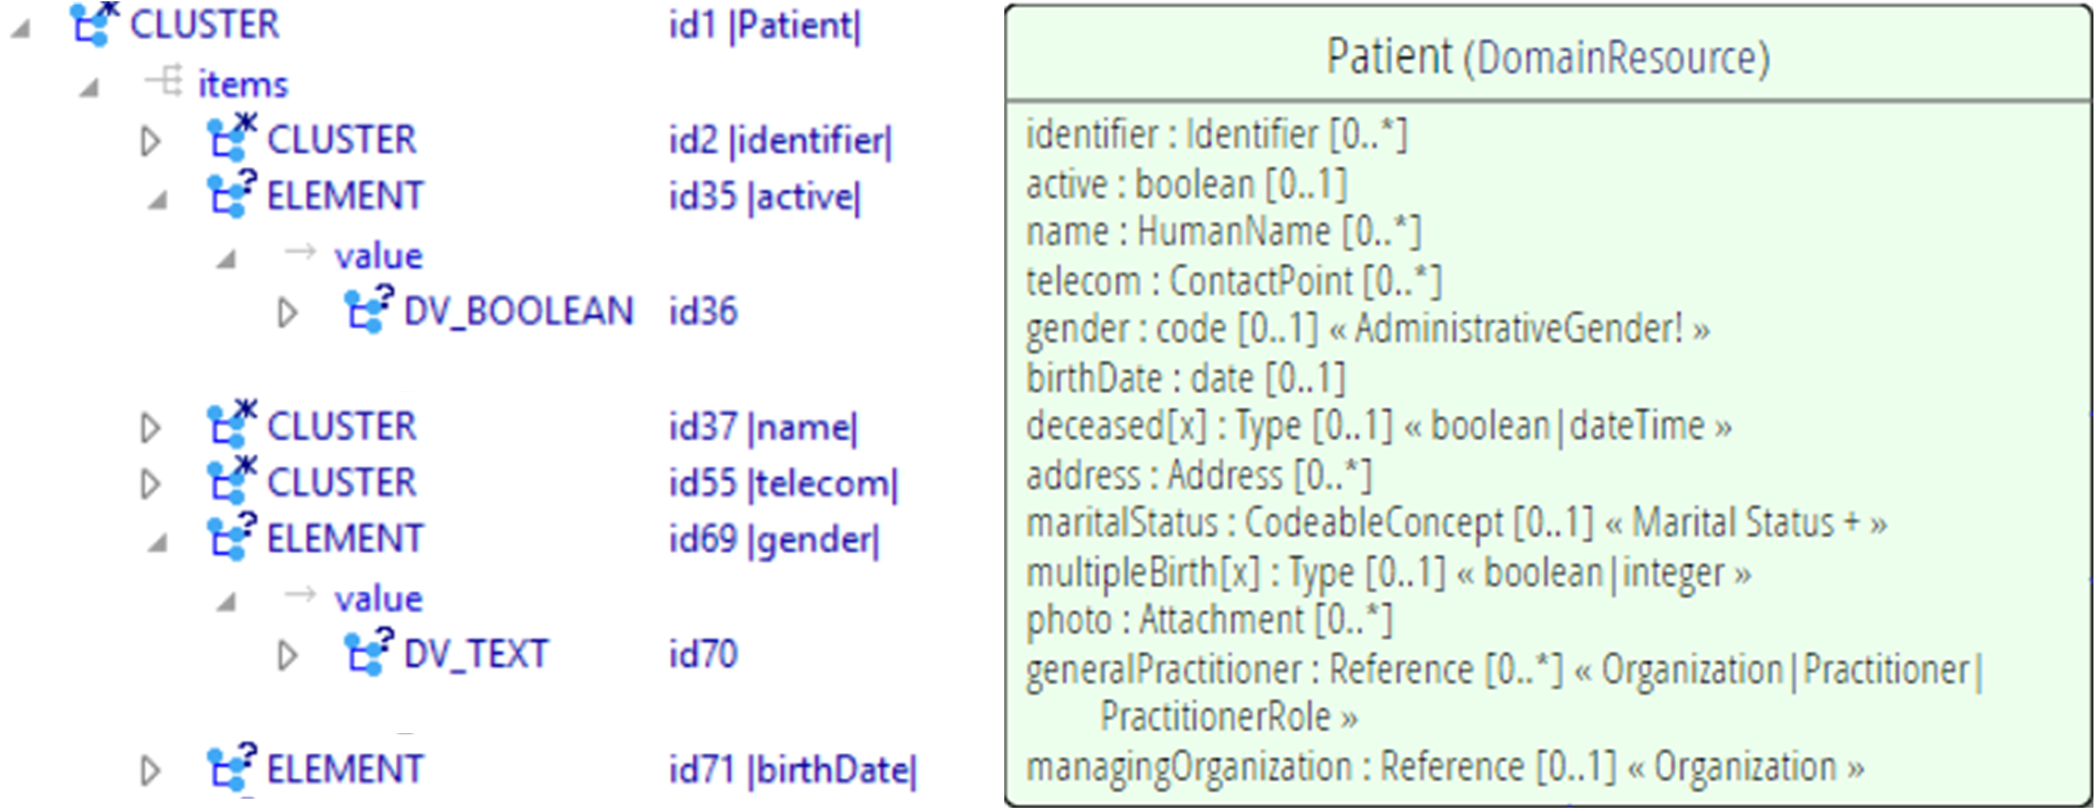
\includegraphics[scale=0.8]{./images/comparison_patient}
  \caption{Comparación de un arquetipo de integración de paciente y un recurso de FHIR paciente.}
  \label{fig:comparison}
\end{figure*}
